\documentclass[a4paper,12pt]{ctexart} 

% First, we usually want to set the margins of our document. For this we use the package geometry.
\usepackage[top = 2.5cm, bottom = 2.5cm, left = 2.5cm, right = 2.5cm]{geometry} 
\usepackage[T1]{fontenc}
\usepackage[utf8]{inputenc}

% The following two packages - multirow and booktabs - are needed to create nice looking tables.
\usepackage{multirow} % Multirow is for tables with multiple rows within one cell.
\usepackage{booktabs} % For even nicer tables.

% As we usually want to include some plots (.pdf files) we need a package for that.
\usepackage{graphicx} 

% The default setting of LaTeX is to indent new paragraphs. This is useful for articles. But not really nice for homework problem sets. The following command sets the indent to 0.
% \usepackage{setspace}
% \setlength{\parindent}{0in}

% Package to place figures where you want them.
\usepackage{float}

% The fancyhdr package let's us create nice headers.
\usepackage{fancyhdr}

\usepackage{amsmath,amsthm,mathabx}

% To make our document nice we want a header and number the pages in the footer.

\pagestyle{fancy} % With this command we can customize the header style.

\fancyhf{} % This makes sure we do not have other information in our header or footer.

\lhead{\footnotesize Probability and Statistics: Section 3.6}% \lhead puts text in the top left corner. \footnotesize sets our font to a smaller size.

%\rhead works just like \lhead (you can also use \chead)
\rhead{\footnotesize 吴梦轩} %<---- Fill in your lastnames.

% Similar commands work for the footer (\lfoot, \cfoot and \rfoot).
% We want to put our page number in the center.
\cfoot{\footnotesize \thepage} 

\begin{document}

\thispagestyle{empty} % This command disables the header on the first page. 

\begin{tabular}{p{15.5cm}}
{\large \bf Probability and Statistics} \\
Southern University of Science and Technology \\ 吴梦轩 \\ 12212006 \\
\hline
\\
\end{tabular}

\vspace*{0.3cm} %add some vertical space in between the line and our title.

\begin{center}
	{\Large \bf Section 3.6}
	\vspace{2mm}

	{\bf 吴梦轩}
		
\end{center}  

\vspace{0.4cm}

\subsubsection*{P79 Q43}

由于$U_1$与$U_2$相互独立,所以$Z = U_1 + U_2$的密度函数为:
\begin{equation*}
	f_Z(z) = \int_{-\infty}^{+\infty} f_{U_1}(u_1)f_{U_2}(z-u_1) \mathrm{d} u_1
\end{equation*}

已知$U_1$与$U_2$的密度函数为:
\begin{equation*}
	f_{U_1}(u_1) = f_{U_2}(u_2) = 
	\begin{cases}
		1 & 0 \leq u_1, u_2 \leq 1 \\
		0 & \text{otherwise}
	\end{cases}
\end{equation*}

所以$S = U_1 + U_2$的密度函数为:
\begin{equation*}
	f_Z(z) = 
	\begin{cases}
		\int_0^z f_{U_1}(u_1)f_{U_2}(z-u_1) \mathrm{d} u_1 = z & 0 \leq z \leq 1 \\
		\int_{z-1}^1 f_{U_1}(u_1)f_{U_2}(z-u_1) \mathrm{d} u_1 = 2-z & 1 < z \leq 2 \\
		0 & \text{otherwise}
	\end{cases}
\end{equation*}

其图像如下:
\begin{center}
	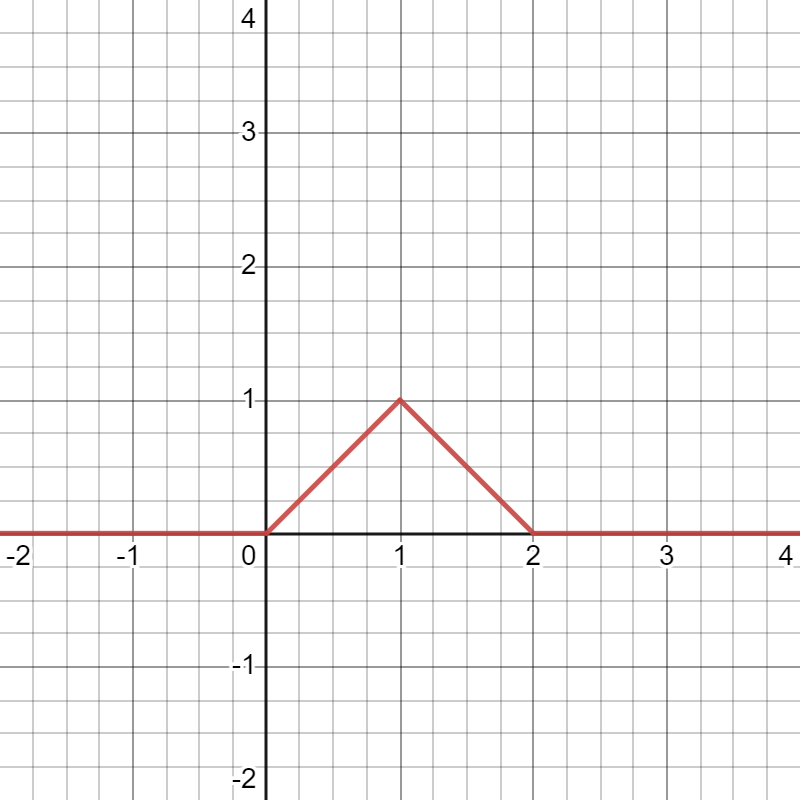
\includegraphics[width=0.5\textwidth]{Plot 1.png}
\end{center}

\subsubsection*{P79 Q44}

令$Z = X + Y$,则有:
\begin{align*}
	P\{Z = 0\} &= P\{X = 0, Y = 0\} = \frac{1}{9} \\
	P\{Z = 1\} &= P\{X = 0, Y = 1\} + P\{X = 1, Y = 0\} = \frac{2}{9} \\
	P\{Z = 2\} &= P\{X = 1, Y = 1\} + P\{X = 0, Y = 2\} + P\{X = 2, Y = 0\} = \frac{1}{3} \\
	P\{Z = 3\} &= P\{X = 1, Y = 2\} + P\{X = 2, Y = 1\} = \frac{2}{9} \\
	P\{Z = 4\} &= P\{X = 2, Y = 2\} = \frac{1}{9}
\end{align*}

所以$X+Y$的频率函数为:
\begin{equation*}
	f_Z(z) = 
	\begin{cases}
		\frac{1}{9} & z = 0 \\
		\frac{2}{9} & z = 1 \\
		\frac{1}{3} & z = 2 \\
		\frac{2}{9} & z = 3 \\
		\frac{1}{9} & z = 4 \\
		0 & \text{otherwise}
	\end{cases}
\end{equation*}

\subsection*{P79 Q51}

令$z = xy$,则有:
\begin{align*}
	F_Z(z) &= \int_{-\infty}^z \int_{-\infty}^{\infty} f \left(x, \frac{z}{x}\right) | J | \mathrm{d} x \mathrm{d} z \\
	&= \int_{-\infty}^z \int_{-\infty}^{\infty} f \left(x, \frac{z}{x}\right) \frac{1}{|x|} \mathrm{d} x \mathrm{d} z \\
	f_Z(z) &= \int_{-\infty}^{\infty} f \left(x, \frac{z}{x}\right) \frac{1}{|x|} \mathrm{d} x
\end{align*}

此时,将变量$x$改名为$y$,有:
\begin{equation*}
	f_Z(z) = \int_{-\infty}^{\infty} f \left(y, \frac{z}{y}\right) \frac{1}{|y|} \mathrm{d} y
\end{equation*}

\subsection*{P79 Q52}

假设两个变量为$[0,1]$上的均匀分布,则有:
\begin{equation*}
	f_X(x) = f_Y(y) =
	\begin{cases}
		1 & 0 \leq x, y \leq 1 \\
		0 & \text{otherwise}
	\end{cases}
\end{equation*}

当$Z \geq 1$时,$Z = \frac{X}{Y}$的分布函数为:
\begin{align*}
	f_Z(z) &= P\{Z \leq z\} \\
	&= P\left\{\frac{X}{Y} \leq z\right\} \\
	&= P\left\{X \leq zY\right\} \\
	&= \int_0^{\frac{1}{z}} \int_0^{zy} f_X(x)f_Y(y) \mathrm{d} x \mathrm{d} y + \int_{\frac{1}{z}}^1 \int_0^1 f_X(x)f_Y(y) \mathrm{d} x \mathrm{d} y \\
	&= \int_0^{\frac{1}{z}} \int_0^{zy} \mathrm{d} x \mathrm{d} y + \int_{\frac{1}{z}}^1 \int_0^1 \mathrm{d} x \mathrm{d} y \\
	&= \frac{1}{2z} + 1 - \frac{1}{z} \\
	&= 1 - \frac{1}{2z}
\end{align*}

当$0 < Z < 1$时,$Z = \frac{X}{Y}$的分布函数为:
\begin{align*}
	f_Z(z) &= \int_0^1 \int_0^{zy} f_X(x)f_Y(y) \mathrm{d} x \mathrm{d} y \\
	&= \int_0^1 \int_0^{zy} \mathrm{d} x \mathrm{d} y \\
	&= \frac{z}{2}
\end{align*}

综上可得:
\begin{equation*}
	f_Z(z) = 
	\begin{cases}
		\frac{\mathrm{d}}{\mathrm{d}z} \frac{z}{2} = \frac{1}{2} & 0 < z < 1 \\
		\frac{\mathrm{d}}{\mathrm{d}z} \left(1 - \frac{1}{2z}\right) = \frac{1}{2z^2} & z \geq 1 \\
		0 & \text{otherwise}
	\end{cases}
\end{equation*}

\subsection*{P80 Q57}

由题可知:
\begin{equation*}
    \begin{bmatrix}
        x_1 \\
        x_2
    \end{bmatrix}
    =
    \begin{bmatrix}
        a_{11} & a_{12} \\
        a_{21} & a_{22}
    \end{bmatrix}
    \begin{bmatrix}
        y_1 \\
        y_2
    \end{bmatrix}
\end{equation*}

\begin{align*}
    f_{Y_1,Y_2}(y_1,y_2) &= \frac{1}{2\pi} e^{-\frac{1}{2}(2y_1^2-2y_1y_2+y_2^2)} \\
    &= \frac{1}{2\pi} e^{-\frac{1}{2} 
    \begin{bmatrix}
        y_1 & y_2
    \end{bmatrix}
    \begin{bmatrix}
        2 & -1 \\
        -1 & 1
    \end{bmatrix}
    \begin{bmatrix}
        y_1 \\
        y_2
    \end{bmatrix}
    } \\
    &= \frac{1}{2\pi} |J| e^{-\frac{1}{2} 
    \begin{bmatrix}
        x_1 & x_2
    \end{bmatrix}
    (J^{-1})^T
    \begin{bmatrix}
        2 & -1 \\
        -1 & 1
    \end{bmatrix}
    J^{-1}
    \begin{bmatrix}
        x_1 \\
        x_2
    \end{bmatrix}
    } \\
    &= \frac{1}{2\pi} e^{-\frac{1}{2} 
    \begin{bmatrix}
        x_1 & x_2
    \end{bmatrix}
    \begin{bmatrix}
        1 & 0 \\
        0 & 1
    \end{bmatrix}
    \begin{bmatrix}
        x_1 \\
        x_2
    \end{bmatrix}
    } \\
    &= \frac{1}{2\pi} e^{-\frac{1}{2}x_1^2-\frac{1}{2}x_2^2}
\end{align*}

因此可知:
\begin{equation*}
    (J^{-1})^T 
    \begin{bmatrix}
        2 & -1 \\
        -1 & 1
    \end{bmatrix}
    J^{-1}
    =
    \begin{bmatrix}
        1 & 0 \\
        0 & 1
    \end{bmatrix}
\end{equation*}

可知当$a_{11} = a_{22} = 1, a_{12} = 0, a_{21} = -1$时,上述方程组成立。

因此$x_1 = y_1, x_2 = y_2 - y_1$。

\subsection*{补充1}

\begin{align*}
	f_{U,V}(u,v) &= f_{X,Y}(x,y) \left| \frac{\partial(x,y)}{\partial(u,v)} \right| \\
	&= \frac{1}{4\pi} e^{-\frac{1}{4} (u^2 + v^2)} 
\end{align*}

其边缘密度函数为:
\begin{align*}
	f_U(u) &= \int_{-\infty}^{+\infty} f_{U,V}(u,v) \mathrm{d} v \\
	&= \int_{-\infty}^{+\infty} \frac{1}{4\pi} e^{-\frac{1}{4} (u^2 + v^2)} \mathrm{d} v \\
	&= \frac{1}{2\sqrt{\pi}} e^{-\frac{1}{4} u^2} \int_{-\infty}^{+\infty} \frac{1}{2\sqrt{\pi}} e^{-\frac{1}{4} v^2} \mathrm{d} v \\
	&= \frac{1}{2\sqrt{\pi}} e^{-\frac{1}{4} u^2} \int_{-\infty}^{+\infty} \frac{1}{\sqrt{2}\sqrt{2\pi}} e^{-\frac{1}{2} \frac{v^2}{\sqrt{2}^2}} \mathrm{d} v \\
	&= \frac{1}{2\sqrt{\pi}} e^{-\frac{1}{4} u^2} 
\end{align*}
同理可知$f_V(v) = \frac{1}{2\sqrt{\pi}} e^{-\frac{1}{4} v^2}$

易知$U$与$V$相互独立,因为$f_{U,V}(u,v) = f_U(u)f_V(v)$。

\subsection*{补充2}

\subsubsection*{(1)}

边缘密度函数为:
\begin{align*}
	f_X(x) &= \int_{0}^{2x} f_{X,Y}(x,y) \mathrm{d} y \\
	&= \int_{0}^{2x} 1 \mathrm{d} y \\
	&= 2x \\
	f_Y(y) &= \int_{\frac{y}{2}}^{1} f_{X,Y}(x,y) \mathrm{d} x \\
	&= \int_{\frac{y}{2}}^{1} 1 \mathrm{d} x \\
	&= 1 - \frac{y}{2}
\end{align*}
\begin{equation*}
	f_X(x) = 
	\begin{cases}
		2x & 0 \leq x \leq 1 \\
		0 & \text{otherwise}
	\end{cases}
\end{equation*}
\begin{equation*}
	f_Y(y) = 
	\begin{cases}
		1 - \frac{y}{2} & 0 \leq y \leq 2 \\
		0 & \text{otherwise}
	\end{cases}
\end{equation*}

\subsubsection*{(2)}

令$u = 2x-y$,则有:
\begin{align*}
	F_Z(z) &= \int_0^z \int_{\frac{u}{2}}^1 f_{X,Y}(x,y) \left| \frac{\partial(x,y)}{\partial(x,u)} \right| \mathrm{d} x \mathrm{d} u \\ 
	&= \int_0^z \int_{\frac{u}{2}}^1 \mathrm{d} x \mathrm{d} u \\
	&= \int_0^z \left(1 - \frac{u}{2}\right) \mathrm{d} u \\
	&= z - \frac{z^2}{4}\ (0 \leq z \leq 2)
\end{align*}

所以$Z$的密度函数为:
\begin{equation*}
	f_Z(z) = \frac{\mathrm{d}}{\mathrm{d}z} \left(z - \frac{z^2}{4}\right) = 1 - \frac{z}{2} \ (0 \leq z \leq 2)
\end{equation*}

\subsubsection*{(3)}

\begin{align*}
	P\{Y < \frac{1}{2} | X < \frac{1}{2}\} &= \frac{P\{Y < \frac{1}{2}, X < \frac{1}{2}\}}{P\{X < \frac{1}{2}\}} \\
	&= \frac{\int_0^{\frac{1}{4}} \int_0^{2x} f_{X,Y}(x,y) \mathrm{d} y \mathrm{d} x + \int_{\frac{1}{4}}^{\frac{1}{2}} \int_{0}^{\frac{1}{2}} f_{X,Y}(x,y) \mathrm{d} y \mathrm{d} x}{\int_0^{\frac{1}{2}} f_X(x) \mathrm{d} x} \\
	&= \frac{\frac{3}{16}}{\frac{1}{4}} \\
	&= \frac{3}{4}
\end{align*}

\end{document}